\chapter{Machine Learning Modeling Review}
\label{ch2}
This section first introduces the fundamentals of machine learning model training and testing, then details the fundamental architectures relevant to this work, and finally reviews the core components in model improvement from examples.
%PyTorch reference \cite{NEURIPS2019_9015}.
%Colah's blog reference \cite{olah}.
\section{Fundamentals of Model Training and Testing}
Figure \ref{fig:simple_model_training} is a simple diagram of how a machine learning model iteratively improves from examples, a process called ``training" or ``learning." Inputs and weights are sent into the model which applies the weights to the inputs to produce a result. The result is analyzed for performance, and based on the performance an update is applied to the weights which will improve model performance.
\begin{figure}[h!]
	\centering
		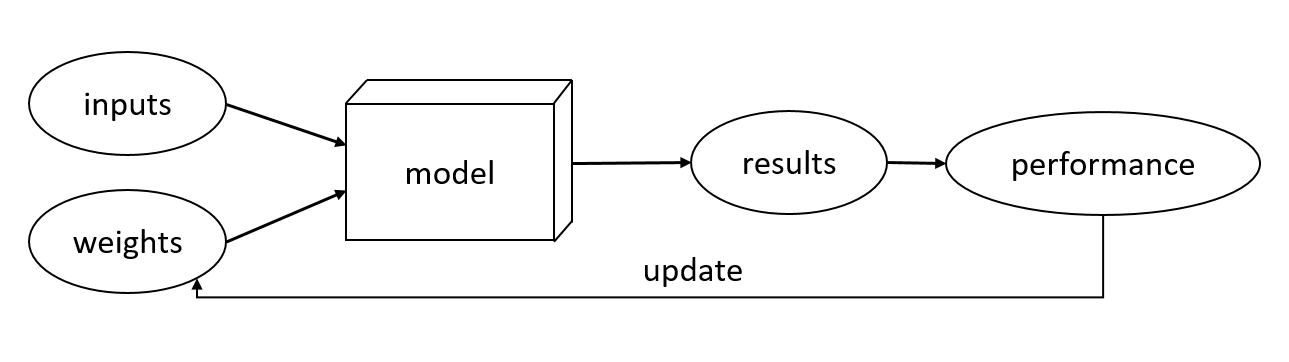
\includegraphics[width=0.99\textwidth]
		{training_process.png}
		\hfill
		\caption{Simple example of machine learning model training .}
		\label{fig:simple_model_training}
\end{figure}
This process is done iteratively until model performance stops improving, i.e., the model has converged to a solution. The final set of weights are the model's trained, or learned, parameters. The modeling described is an example of ``supervised learning" in which a set of inputs is associated with a known (truth) value trying to be modeled. The performance analysis compares the model output with the truth value.

The trained model is then ready for testing, or inference, on another set of inputs. Figure \ref{fig:simple_model_testing} illustrates this process.
\begin{figure}[h!]
	\centering
	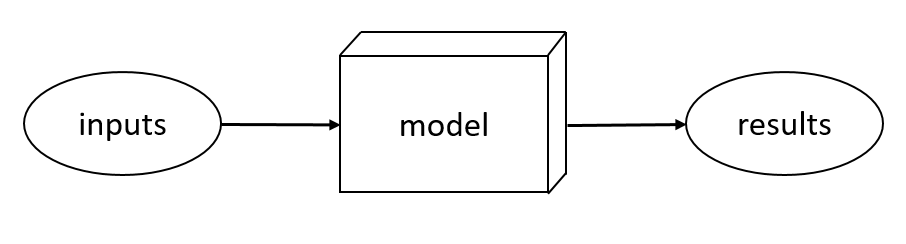
\includegraphics[width=0.99\textwidth]
	{testing_process.png}
	\hfill
	\caption{Simple example of machine learning model testing.}
	\label{fig:simple_model_testing}
\end{figure}
The learned parameters from the training process are static in the model and are applied to the inputs to produce a result. The test inputs must be in the same format of the inputs used during training. While not required, it's highly desirable for the test inputs to be of similar values as the train inputs.

\section{Machine Learning Model Architectures}
\subsection{Multilayer Perceptron}
The \ac{MLP} is a feedforward \ac{ANN} consisting of at least three layers of nodes: an input layer, a hidden layer, and an output layer. The number of hidden layers in an \ac{MLP} is adjustable to be greater than one. Each node in the \ac{MLP} is a value, also called the node's activation. Each node in the input layer represents an input variable. Each node in the hidden and output layers represent the weighted sum of the activations from the previous layer. The \ac{MLP} is described as ``fully-connected" because each node in one layer connects with a specific weight $w_{ij}$ to every node in the following layer.

Figure \ref{fig:architecture_MLP_simple} is a simple 2-layer \ac{MLP} associated with the problem addressed in this work. The input layer, which is not counted towards the depth (number of layers) of the \ac{NN}, is five nodes wide. Each input node represents a weather variable: temperature, pressure, relative humidity, wind speed, and solar irradiance.
\begin{figure}[h!]
	\centering
	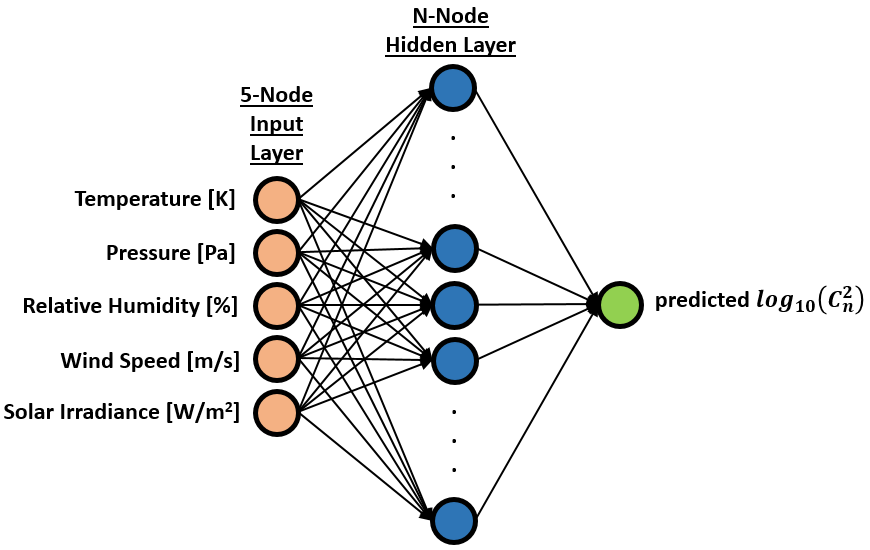
\includegraphics[width=0.99\textwidth]
	{architecture_MLP_simple.png}
	\hfill
	\caption{Simple MLP (multi-layer perceptron) to predict $log_{10}(C_{n}^{2})$ from weather inputs.}
	\label{fig:architecture_MLP_simple}
\end{figure}
The input layer is fully-connected to the only hidden layer which is $N$-nodes wide. In application the researcher sets $N$. The hidden layer is described as ``hidden" because its nodes are buried in the model, i.e., are not part of the \emph{inputs} or the \emph{outputs}. The arrows from input layer to hidden layer in Figure \ref{fig:architecture_MLP_simple} illustrate the concept of an \ac{MLP} being fully-connected: an arrow points from each node in the input layer to each node in the hidden layer. This is further shown in the full connection between the hidden layer and output layer which has only a single node. The \ac{NN} in Figure \ref{fig:architecture_MLP_simple} is a single-output \emph{regression} \ac{MLP} because the output layer is a single node of \emph{continuous} values. Specifically, the \ac{MLP} in Figure \ref{fig:architecture_MLP_simple} models the relationship between a set of weather inputs and $log_{10}{C_{n}^{2}}$ value. The other major \ac{NN} type is \emph{classification} which predicts/classifies \emph{discrete} values or labels. Only regression \ac{NN} is used in this work.

%Figure \ref{fig:architecture_MLP_forecast} is an example of a 3-layer multi-output regression \ac{MLP} related to the problem addressed in this work.
%\begin{figure}[h!]
%	\centering
%	\includegraphics[width=0.99\textwidth]
%	{architecture_MLP_forecast.png}
%	\hfill
%	\caption{MLP to forecast eight time steps of $log_{10}(C_{n}^{2})$ from multiple time steps of weather inputs.}
%	\label{fig:architecture_MLP_forecast}
%\end{figure}

When fully-connected, the activations of a layer of nodes are calculated from the prior layer's node activations by
\begin{equation} \label{eq:MLP}
	\vec{y} = \sigma \left(\textbf{W}\vec{x} + \vec{b}\right)
\end{equation}
where $\vec{x}$ is the input vector of prior layer node activations, $\vec{y}$ is the output vector of next layer node activations, $\textbf{W}$ and $\vec{b}$ are the learnable matrix weights and vector biases, and $\sigma$ is a non-linear activation function. In matrix notation, Equation \ref{eq:MLP} for a 2-node layer fully-connected to another 2-node layer is written
\begin{equation} \label{eq:MLP_matrix}
	\begin{bmatrix}
		y_{1} \\
		y_{2}
	\end{bmatrix}
	= \sigma \left(
	\begin{bmatrix}
		w_{1,1} & w_{1,2} \\
		w_{2,1} & w_{2,2}
	\end{bmatrix}
	\begin{bmatrix}
		x_{1} \\
		x_{2}
	\end{bmatrix}
	+
	\begin{bmatrix}
		b_{1} \\
		b_{2}
	\end{bmatrix}
	\right).
\end{equation}
The matrix-vector product $\textbf{W}x$ is the weighted sum of the learnable weights and the input layer node activations. The notation of the weight matrix elements $w_{ij}$ is such that $i$ is the $i^{th}$ node of the output layer and $j$ is the $j^{th}$ node of the input layer. The elements in the bias vector $\vec{b}$ are similar to the constant $b$ of a linear function
\[
y = ax + b
\]
that allows the model to best fit for the given data.

The matrix-vector product of the weights and inputs and the addition of the bias vector are purely linear which constrains the model to learn only linear relationships. The $\sigma$ in Equations \ref{eq:MLP} and \ref{eq:MLP_matrix} is a non-linear activation function applied element-wise to the values calculated from 
\[
\begin{bmatrix}
	w_{1,1} & w_{1,2} \\
	w_{2,1} & w_{2,2}
\end{bmatrix}
\begin{bmatrix}
	x_{1} \\
	x_{2}
\end{bmatrix}
+
\begin{bmatrix}
	b_{1} \\
	b_{2}
\end{bmatrix}
\]
to allow the model to learn non-linear relationships. The particular non-linear activation function $\sigma$ is the sigmoid which squishes its argument between 0 (zero) and 1 by
\begin{equation} \label{eq:sigmoid}
	\text{sigmoid}\left(x\right) = \sigma \left(x\right) = \frac{1}{1 + \exp \left(-x\right)}.
\end{equation}
Figure \ref{fig:activation_functions_a} \cite{NEURIPS2019_9015} illustrates the effect of the sigmoid activation function. Two additional activation functions used in this work are the hyperbolic tangent ($\tanh$) defined as
\begin{equation} \label{eq:tanh}
	\tanh \left(x\right) = \frac{\exp \left(x\right) - \exp \left(-x\right)}{\exp \left(x\right) + \exp \left(-x\right)},
\end{equation}
and the \ac{ReLU} defined as
\begin{equation} \label{eq:relu}
	\text{ReLU} \left(x\right) = \max \left(0, x\right).
\end{equation}
The $\tanh$ is similar to the sigmoid but squishes the input to between -1 and +1 as illustrated in Figure \ref{fig:activation_functions_b}. The \ac{ReLU} is a piecewise linear function that returns a positive input as itself but returns 0 (zero) if the input is negative as shown in Figure \ref{fig:activation_functions_c}. The \ac{RNN} architectures explored in this work use the sigmoid and $\tanh$ activation functions, and the \ac{MLP} architectures use the ReLU which is the most commonly used activation function in deep learning models.
\begin{figure}[p!]
 	\centering
 	\subfloat[Telescope setup\label{fig:activation_functions_a}]{
 		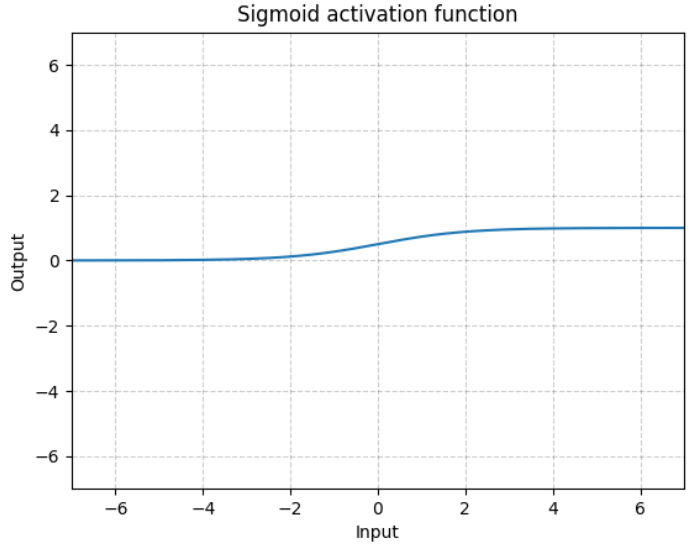
\includegraphics[width=0.49\textwidth]
 		{activation_function_Sigmoid.png}
 	}
 	\hfill
 	\subfloat[Telescope setup\label{fig:activation_functions_b}]{
 		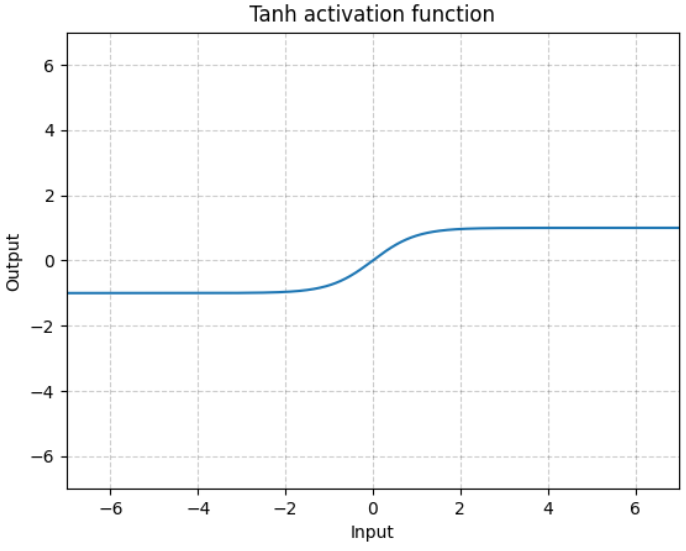
\includegraphics[width=0.485\textwidth]
 		{activation_function_tanh.png}
 	}
 	\subfloat[Wide view of target\label{fig:activation_functions_c}]{
 		\includegraphics[width=0.49\textwidth]
 		{activation_function_ReLU.png}
 	}
 	\hfill
 	\caption{Sigmoid ($\sigma$), hyperbolic tangent ($\tanh$) and Rectified Linear Unit (ReLU) activation functions}
 	\label{fig:activation_functions}
\end{figure}





\clearpage

\subsection{Recurrent Neural Networks}
\begin{figure}[h!]
	\centering
	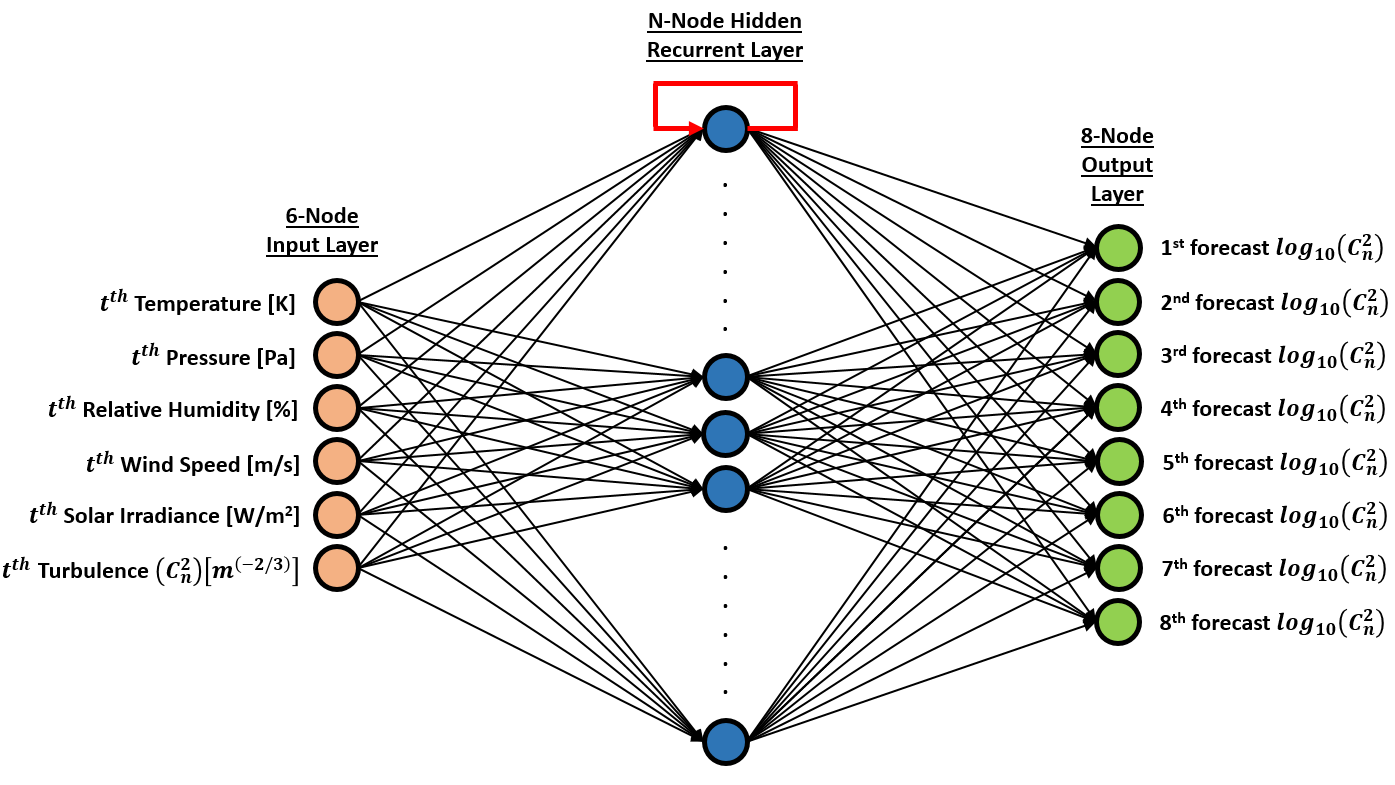
\includegraphics[width=0.99\textwidth]
	{architecture_RNN_single_layer.png}
	\hfill
	\caption{Single-layer RNN architecture to forecast eight time steps of $log_{10}(C_{n}^{2})$ from multiple time steps of weather inputs processed by the recurrent layer.}
	\label{fig:architecture_RNN_single_layer}
\end{figure}

\begin{figure}[h!]
	\centering
	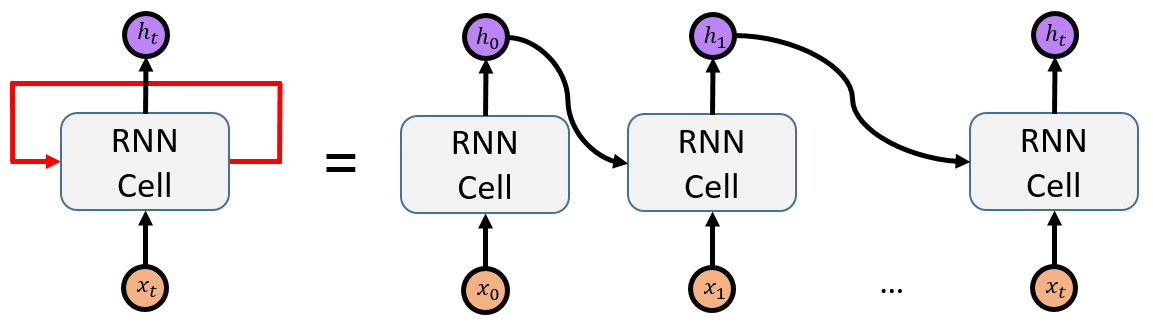
\includegraphics[width=0.99\textwidth]
	{architecture_RNN_single_layer_unrolled.png}
	\hfill
	\caption{Unrolled single-layer RNN}
	\label{fig:architecture_RNN_single_layer_unrolled}
\end{figure}

\begin{figure}[h!]
	\centering
	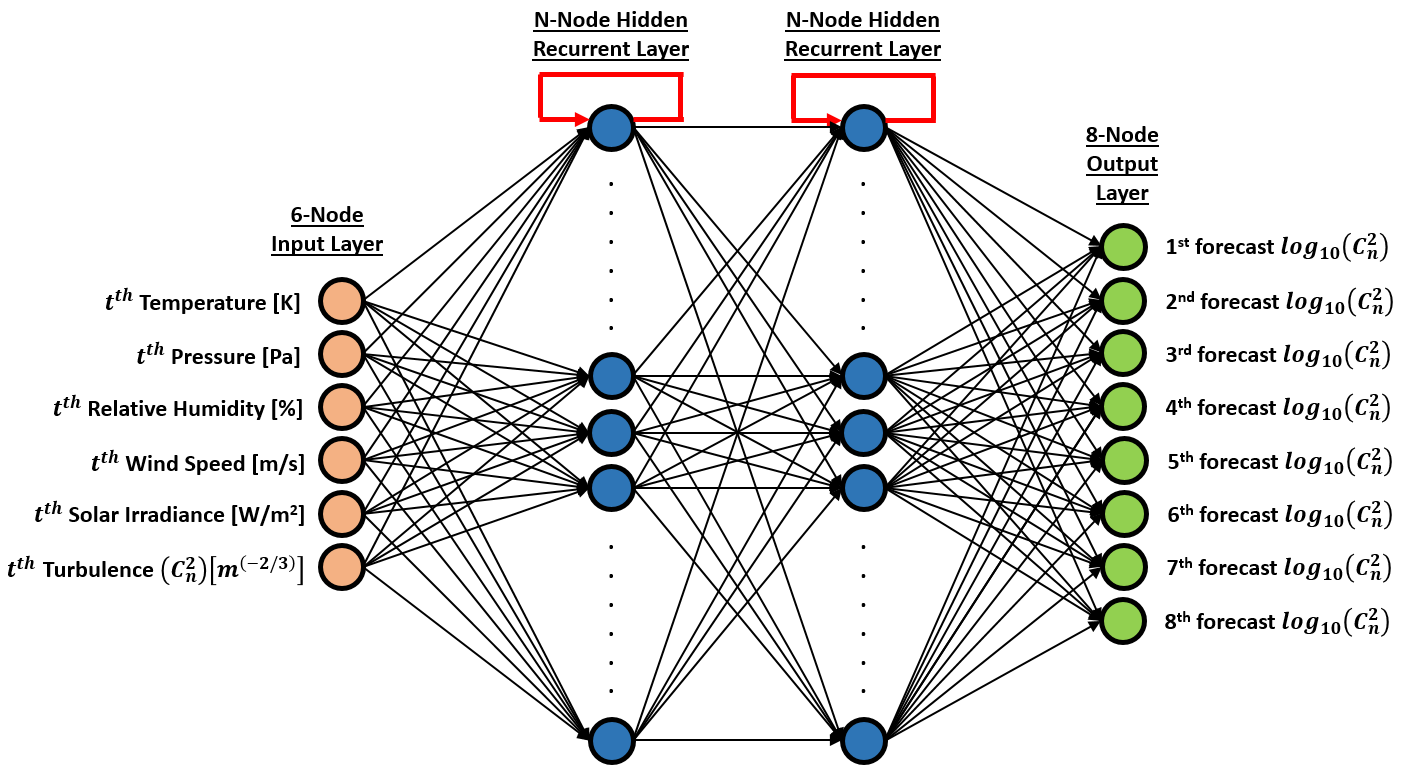
\includegraphics[width=0.99\textwidth]
	{architecture_RNN_multi_layer.png}
	\hfill
	\caption{Multi-layer RNN architecture to forecast eight time steps of $log_{10}(C_{n}^{2})$ from multiple time steps of weather inputs processed by the recurrent layers.}
	\label{fig:architecture_RNN_multi_layer}
\end{figure}

\begin{figure}[h!]
	\centering
	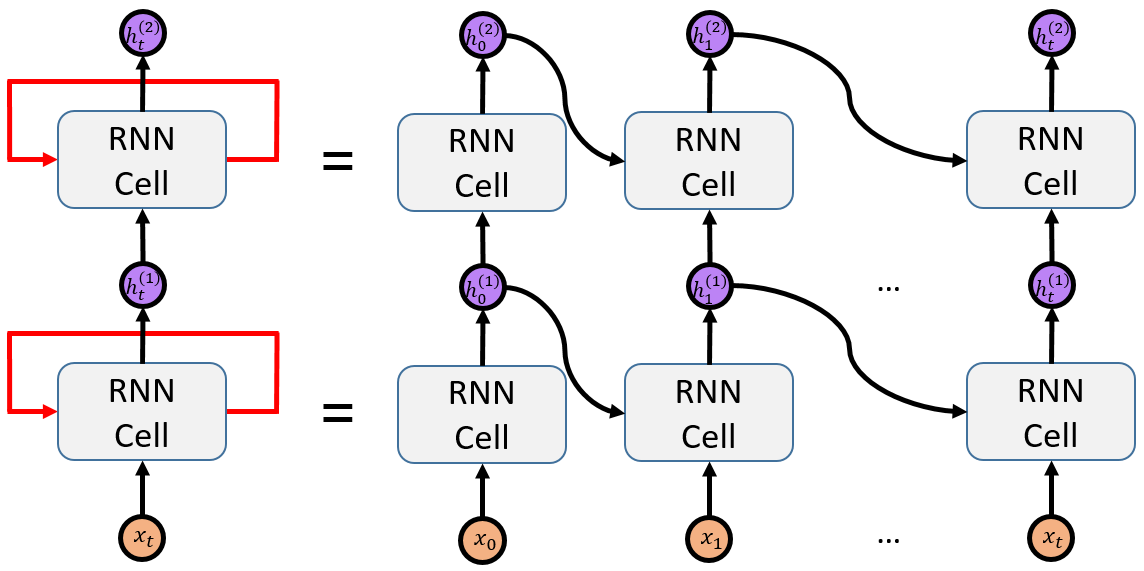
\includegraphics[width=0.99\textwidth]
	{architecture_RNN_multi_layer_unrolled.png}
	\hfill
	\caption{Unrolled multi-layer RNN}
	\label{fig:architecture_RNN_multi_layer_unrolled}
\end{figure}

\subsubsection{Simple RNN}
A \ac{RNN} is a neural network that operates on a variable-length sequence. The \ac{RNN} processes the sequence input with a hidden state $h$ whose activation (value) at each time $t$ is dependent on the activation of the previous time. At each time step $t$ the hidden state $h_{t}$ of the \ac{RNN} is updated by
\begin{equation} \label{eq:RNN}
	h_{t} = \tanh\left(W_{ih}x_{t} + b_{ih} + W_{hh}h_{\left(t-1\right)} + b_{hh}\right)
\end{equation}
where $x_{t}$ is the input at time $t$, $h_{\left(t-1\right)}$ is the hidden state of the previous layer at time $t-1$ or the initial state at time 0 (zero), $W_{ih}$ is the learnable input-hidden weights, $b_{ih}$ is the learnable input-hidden bias, $W_{hh}$ is the learnable hidden-hidden weights, and $b_{hh}$ is the learnable hidden-hidden bias \cite{NEURIPS2019_9015}.

\begin{figure}[h!]
	\centering
	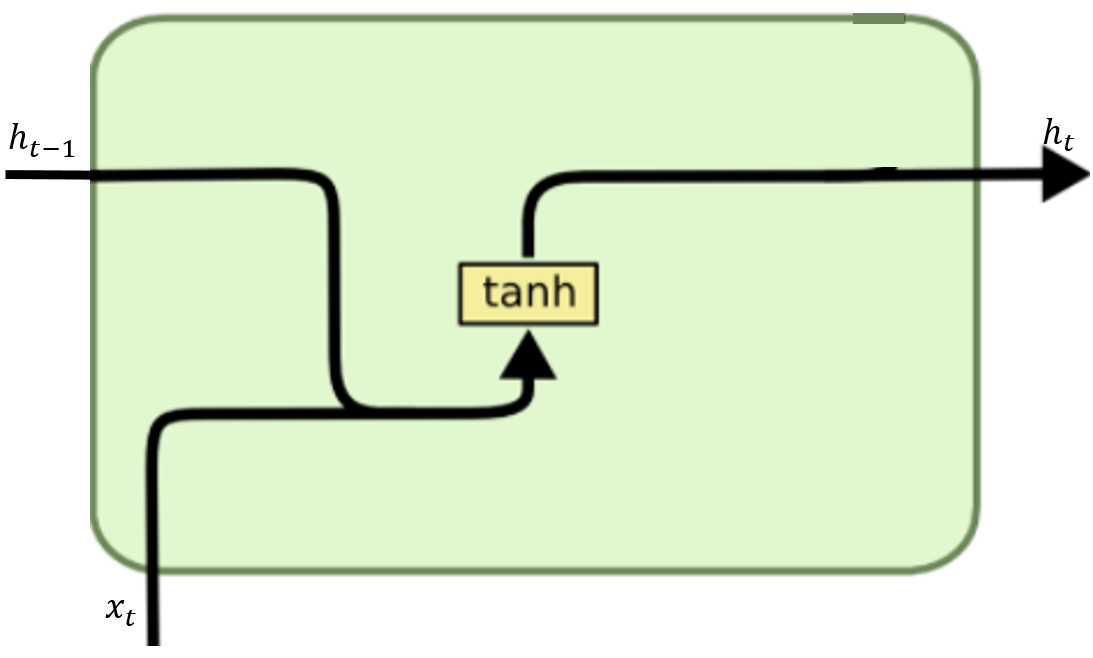
\includegraphics[width=0.7\textwidth]
	{cell_RNN.png}
	\hfill
	\caption{Simple RNN cell}
	\label{fig:cell_RNN}
\end{figure}

\clearpage

\subsubsection{LSTM-RNN}
\ac{LSTM-RNN}. For each element in the input sequence, each layer computes the following function:
\begin{align}
	i_{t} &= \sigma\left(W_{ii}x_{t} + b_{ii} + W_{hi}h_{\left(t-1\right)} + b_{hi}\right) \label{eq:LSTM1} \\
	f_{t} &= \sigma\left(W_{if}x_{t} + b_{if} + W_{hf}h_{\left(t-1\right)} + b_{hf}\right) \label{eq:LSTM2} \\
	g_{t} &= \tanh\left(W_{ig}x_{t} + b_{ig} + W_{hg}h_{\left(t-1\right)} + b_{hg}\right) \label{eq:LSTM3} \\
	o_{t} &= \sigma\left(W_{io}x_{t} + b_{io} + W_{ho}h_{\left(t-1\right)} + b_{ho}\right) \label{eq:LSTM4} \\
	c_{t} &= f_{t} \odot c_{\left(t-1\right)} + i_{t} \odot g_{t} \label{eq:LSTM5} \\
	h_{t} &= o_{t} \odot \tanh\left(c_{t}\right) \label{eq:LSTM6}
\end{align}
where $h_{t}$ is the hidden state at time $t$, $c_{t}$ is the cell state at time $t$, $x_{t}$ is the input at time $t$, $h_{\left(t-1\right)}$ is the hidden state of the layer at time $t-1$ or the initial state at time 0 (zero), and $i_{t}$, $f_{t}$, $g_{t}$, and $o_{t}$ are the input, forget, cell, and output gates, respectively. $W_{ii}$, $W_{if}$, $W_{ig}$, and $W_{io}$ are the learnable input-hidden weights for the input, forget, cell, and output gates. $\sigma$ is the sigmoid function, and $\odot$ is the Hadamard (element-wise) product \cite{NEURIPS2019_9015}.

\begin{figure}[h!]
	\centering
	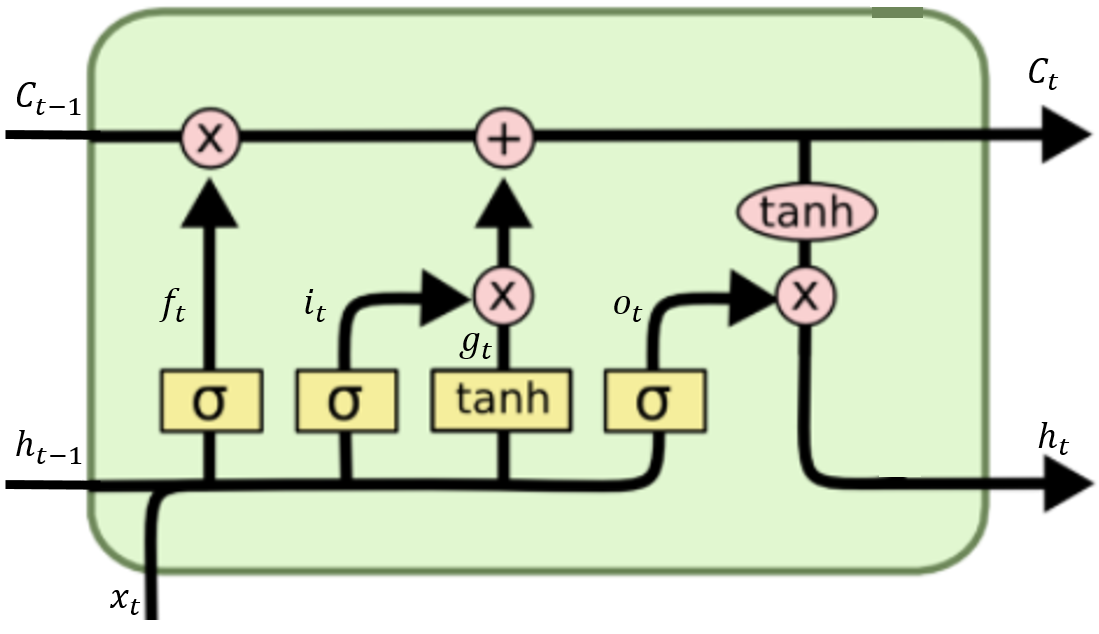
\includegraphics[width=0.7\textwidth]
	{cell_LSTM.png}
	\hfill
	\caption{LSTM-RNN cell}
	\label{fig:cell_LSTM}
\end{figure}

\subsubsection{GRU-RNN}
\ac{GRU-RNN}. For each element in the input sequence, each layer computes the following function:
\begin{align}
	r_{t} &= \sigma\left(W_{ir}x_{t} + b_{ir} + W_{hr}h_{\left(t-1\right)} + b_{hr}\right) \label{eq:GRU1} \\
	z_{t} &= \sigma\left(W_{iz}x_{t} + b_{iz} + W_{hz}h_{\left(t-1\right)} + b_{hz}\right) \label{eq:GRU2} \\
	n_{t} &= \tanh\left(W_{in}x_{t} + b_{in} + r_{t} \odot \left(W_{hn}h_{\left(t-1\right)} b_{hn}\right)\right) \label{eq:GRU3} \\
	h_{t} &= \left(1 - z_{t}\right) \odot n_{t} + z_{t} \odot h_{\left(t-1\right)} \label{eq:GRU4}
\end{align}
where $h_{t}$ is the hidden state at time $t$, $x_{t}$ is the input at time $t$, $h_{\left(t-1\right)}$ is the hidden state of the layer at time $t-1$ or the initial hidden state at time 0 (zero), and $r_{t}$, $z_{t}$, and $n_{t}$ are the reset, update, and new gates, respectively. $W_{ir}$, $W_{iz}$ and $W_{in}$ are the learnable input-hidden weights for the reset, update, and new gates, respectively, and are of shape $numlayers \times 3hiddensize \times inputsize$. $W_{hr}$, $W_{hz}$ and $W_{hn}$ are the learnable hidden-hidden weights for the reset, update, and new gates, respectively, and are of shape $numlayers \times 3hiddensize \times inputsize$. $b_{ir}$, $b_{iz}$, and $b_{in}$ are the learnable input-hidden biases of the reset, update, and new gates, respectively. $b_{hr}$, $b_{hz}$, and $b_{hn}$ are the learnable hidden-hidden biases of the reset, update, and new gates, respectively. $\sigma$ is the sigmoid function, and $\odot$ is the Hadamard (element-wise) product \cite{NEURIPS2019_9015}. 

\begin{figure}[h!]
	\centering
	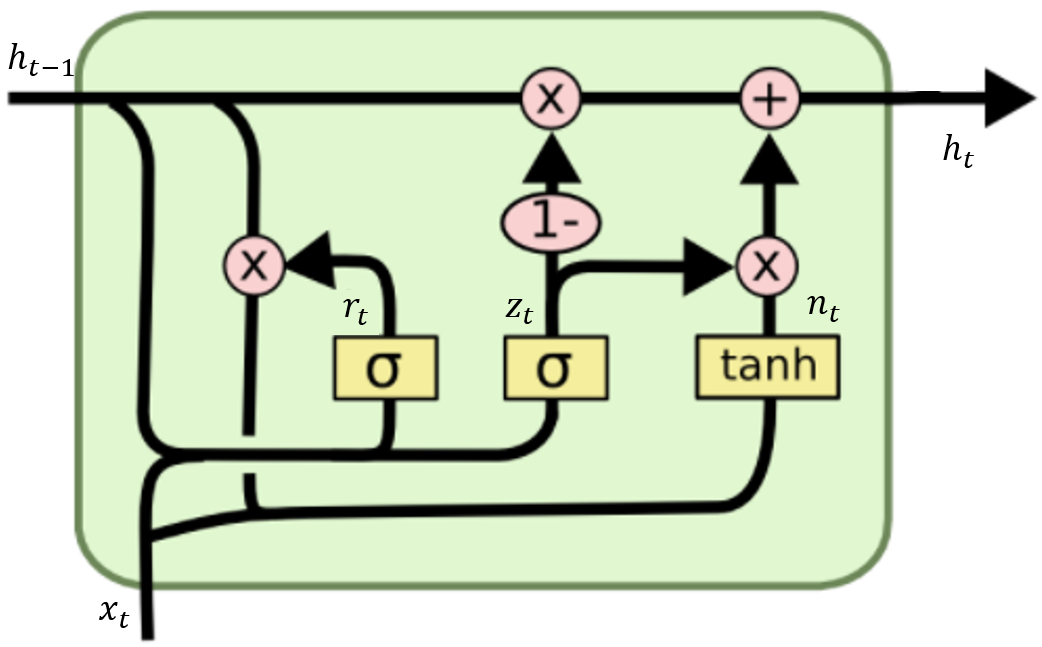
\includegraphics[width=0.7\textwidth]
	{cell_GRU.png}
	\hfill
	\caption{GRU-RNN cell}
	\label{fig:cell_GRU}
\end{figure}

\section{Optimization and Loss Function}
Neural networks are a collection of nested functions that are executed on some input data. These functions are defined by \emph{parameters} (weights and biases). The training of a neural network is the process of updating the parameters to reduce the loss between network outputs and truth values. Training happens in two steps. The first step is forward propagation in which the network makes a prediction by passing input values through its functions (applying the weights and biases). The second step is backward propagation where the network adjusts its parameters proportionate to the error in its prediction. The network does this by moving backwards through the network from the output, collecting the derivatives of the error with respect to the parameters of the functions and optimizing the parameters using gradient descent. The derivatives of the error with respect to the parameters are called gradients. PyTorch's automatic differentiation engine \textit{autograd} handles this entire process \cite{NEURIPS2019_9015}.

Follow 3Blue1Brown video but with my own images and notations. Start with a 1x1 then move to a 2x2 network?
``These chain rule expressions give you the derivatives that determine each component in the gradient that helps minimize the loss of the network by repeatedly stepping downhill." - 3Blue1Brown

\section{Chapter Summary?}